%! TeX program = xelatex
\documentclass[fontset=none]{ctexart}
%===================================
% note-setup-leftsidebox.tex
% huanengchen@foxmail.com 2025-08-12
%===================================
% 参考:https://tex.stackexchange.com/questions/59702/suggest-a-nice-font-family-for-my-basic-latex-template-text-and-math

%===================================
% 页面和间距
%===================================

\usepackage[a4paper, margin=1in]{geometry} % 具体设置参考 geometry 宏包
\setlength{\parindent}{0pt} % 取消首行缩进
\usepackage{parskip} % 形成段落间的间距
\linespread{1.25} % 修改行距

%===================================
% 编辑体验
%===================================

\usepackage{float} % 优化浮动体
\usepackage[shortlabels,inline]{enumitem} % 优化列表
\usepackage{appendix} % 优化附录

%===================================
% 表格
%===================================

\usepackage{booktabs, multirow, multicol}
\usepackage{tabularx} % 表格自动换行,调整表格宽度 
\usepackage{makecell} % 单元格内换行
\usepackage{threeparttable} % 给表格添加脚注,参考:https://tex.stackexchange.com/questions/6090/clickable-table-footnote
\usepackage{ltablex} % 跨页表格

%===================================
% 参考文献
%===================================

\usepackage[sort&compress]{gbt7714} % 参考文献样式
\bibliographystyle{gbt7714-numerical} % 顺序编码制

%===================================
% 颜色
%===================================

\usepackage[dvipsnames, x11names, table]{xcolor} % 参考:https://tex.stackexchange.com/questions/659036/option-selecting-named-colours-provided-by-the-xcolor-package

%===================================
% 支持插入图片及子图
%===================================

\usepackage{graphicx}
\graphicspath{
    {./figure/}{./figures/}{./image/}{./images/}{./graphic/}{./graphics/}{./picture/}{./pictures/}
} % 用于存放图片的目录,这样引用图片的时候就不需要指定目录
\usepackage{subcaption}

%===================================
% 算法和伪代码
%===================================

\usepackage[linesnumbered, ruled, longend, lined]{algorithm2e} % 参考 algorithm2e 宏包文档
\DontPrintSemicolon % 不打印分号
\setlength{\algomargin}{2em} % 设置算法缩进使得行号在线框内
\renewcommand{\CommentSty}[1]{\normalsize\textit{#1}} % 设置注释的字体样式为意大利斜体,字体大小为 \normalsize

%===================================
% 代码
%===================================

\usepackage{minted} % 参考 minted 宏包文档

% 代码行号样式
\renewcommand{\theFancyVerbLine}{
\sffamily
\textcolor{gray}{
\footnotesize\oldstylenums{
\arabic{FancyVerbLine}}}}

% 行间代码环境
\setminted{
    style=colorful, % 设置代码风格,可选的代码风格参考:https://pygments.org/styles/
    numbers=left, % 显示行号
    numbersep=2pt, % 行号与代码的距离
    mathescape, % 允许在代码注释中使用数学公式
    breaklines, % 允许代码自动断行 
    fontsize=\footnotesize, % 设置代码字体大小
    frame=single, % 设置代码框
    framerule=0.5pt, % 设置代码框线宽
    resetmargins, % 重置代码边距
}

% 行内代码环境
\setmintedinline{
    style=colorful, % 设置代码风格,可选的代码风格参考:https://pygments.org/styles/
    fontsize=\footnotesize, % 设置代码字体大小
    breakanywhereinlinestretch=0.01em, % 允许行内代码在任意位置断行
    breaklines, % 允许行内代码自动断行
}

%===================================
% 超链接
%===================================

\usepackage{hyperref}
\hypersetup{
    bookmarksopen=true, % 启用书签
    colorlinks=true, % 启用颜色
    linkcolor=red, % 内部链接的颜色
    linktoc=all, % 设置目录中的页码和标题都能够跳转
    citecolor=violet, % 引用链接的颜色
    urlcolor=magenta, % 外部链接的颜色
}

%===================================
% 数学公式
%===================================

\usepackage{amsmath, amsthm, amsfonts, amssymb} % 用于加载数学公式、花体字母和数学字符
\usepackage{mathtools}
\usepackage{mathrsfs}
\usepackage{bm}
\usepackage{extarrows}
\usepackage[noabbrev]{cleveref} % 多公式引用,必须放在 hyperref 宏包的后面,参考:https://tex.stackexchange.com/questions/314217/how-i-can-refer-multiple-equation-in-latex

\allowdisplaybreaks[1] % 多行公式换页,1 为尽量避免换页
\crefname{equation}{}{} % 设置非首字母大写的引用格式
\Crefname{equation}{}{} % 设置首字母大写的引用格式
\crefrangeformat{equation}{(#3#1#4)-(#5#2#6)} % 多公式引用的格式

%===================================
% 边注
%===================================

% 设置边注的字体大小
\let\oldmarginpar\marginpar
\renewcommand{\marginpar}[1]{\oldmarginpar{\footnotesize #1}}

%===================================
% 页脚和页眉
%===================================

\usepackage{fancyhdr} % 参考:https://tex.stackexchange.com/questions/732462/chapter-number-in-the-header-with-chapter/732464?noredirect=1#comment1824660_732464 
\usepackage{lastpage} % 获取总页码
\setlength{\headheight}{13pt} % 设置页眉高度

% 重新定义 \author 和 \date 命令用于页眉
\makeatletter
\let\oldauthor\author
\renewcommand{\author}[1]{\oldauthor{#1}\def\myauthor{#1}}
\let\olddate\date
\renewcommand{\date}[1]{\olddate{#1}\def\mydate{#1}}
\makeatother

% 详细参数参考 fancyhdr 宏包
\pagestyle{fancy} % 设置文档的页面样式为 fancy,这意味着页眉和页脚将使用 fancyhdr 宏包提供的自定义格式
\fancyhf{} % 清空原本的页脚页眉样式

% 自定义页眉
\fancyhead[L]{\myauthor} % 左侧显示作者
\fancyhead[R]{\mydate} % 右侧显示日期

\cfoot{\thepage\ / \pageref*{LastPage}} % 自定义页脚,参考:https://tex.stackexchange.com/questions/227/how-can-i-add-page-of-on-my-document

%===================================
% 字体
%===================================

\usepackage[T1]{fontenc} % 改善文档中西欧语言的显示效果
\usepackage{anyfontsize}
\usepackage{lmodern} % lmodern字体
\usepackage{libertine} % Linux Libertine 字体系列(衬线字体)

% 中文字体,具体设置参考 ctex 宏包
\setCJKmainfont{LXGWWenKaiScreen.ttf}[ % 设置中文主字体为霞鹜文楷屏幕舒适版
    Path=./fonts/,
    BoldFont=FZHTJW.TTF, % 设置粗体为方正黑体
    ItalicFont=FZKTJW.TTF, % 设置斜体为方正楷体
]
\setCJKsansfont{FZHTJW.TTF}[ % 设置无衬线字体为方正黑体
    Path=./fonts/,
    AutoFakeBold=1.5,  % 生成粗体效果
    ItalicFont=FZFSJW.TTF, % 设置斜体为方正仿宋
]
\setCJKmonofont{LXGWWenKaiMonoScreen.ttf}[ % 设置等宽字体为霞鹜文楷等宽屏幕舒适版
    Path=./fonts/,
    AutoFakeBold=1.5,  % 生成粗体效果
    ItalicFont=FZSSJW.TTF, % 设置斜体为方正书宋
] 

% 英文字体,具体设置参考 fontspec 宏包
\setmonofont{MapleMono-NF-CN}[ % 设置英文等宽字体
    Path=./fonts/, % 指定字体文件所在的目录
    Extension=.ttf, % 字体文件后缀
    UprightFont=*-Regular, % 正常字体
    BoldFont=*-Bold, % 加粗
    ItalicFont=*-Italic, % 斜体
    BoldItalicFont=*-BoldItalic, % 粗斜体
]

%===================================
% 定理盒子
%===================================

% 修改 proof 环境的引导词为 Proof,样式为加粗无斜体
\renewcommand*{\proofname}{\normalfont\bfseries Proof}

% 导入 thmtools 宏包,使用 \declaretheorem 命令来定义各种定理环境(比 \newtheorem 命令更加方便)
\usepackage{thmtools}

% 定义环境使用的 `\declaretheorem` 命令参数包括:
% - `style`: 定理环境样式,amsthm 内置的样式包括
%   - plain(默认):引导词是正体,内容是斜体
%   - definition:引导词和内容都是正体
%   - remark:引导词是斜体,内容是正体
% - `name`:显示在正文中的引导词(不等于环境的名称)
% - `numbered`:是否开启编号
% - `numberwithin`、`sibling`:定义编号规则,例如:
%   - `numberwithin=section`:基于 section 编号
%   - `sibling=theorem`:共享 `theorem` 环境的编号

% 采用 plain 样式,定义 `theorem`/`theorem*`、`proposition`/`proposition*`、`corollary`/`corollary*`、`lemma`/`lemma*`、`claim`/`claim*` 环境

\declaretheorem[style=plain, name=Theorem, numbered=yes, numberwithin=section]{theorem}
\declaretheorem[style=plain, name=Theorem, numbered=no]{theorem*}

\declaretheorem[style=plain, name=Proposition, numbered=yes, sibling=theorem]{proposition}
\declaretheorem[style=plain, name=Proposition, numbered=no]{proposition*}

\declaretheorem[style=plain, name=Corollary, numbered=yes, sibling=theorem]{corollary}
\declaretheorem[style=plain, name=Corollary, numbered=no]{corollary*}

\declaretheorem[style=plain, name=Lemma, numbered=yes, sibling=theorem]{lemma}
\declaretheorem[style=plain, name=Lemma, numbered=no]{lemma*}

\declaretheorem[style=plain, name=Claim, numbered=yes, sibling=theorem]{claim}
\declaretheorem[style=plain, name=Claim, numbered=no]{claim*}

% 采用 definition 样式,定义 `definition`/`definition*`、`example`/`example*`、`problem`/`problem*` 环境

\declaretheorem[style=definition, name=Definition, numbered=yes, numberwithin=section]{definition}
\declaretheorem[style=definition, name=Definition, numbered=no]{definition*}

\declaretheorem[style=definition, name=Example, numbered=yes, numberwithin=section]{example}
\declaretheorem[style=definition, name=Example, numbered=no]{example*}

\declaretheorem[style=definition, name=Problem, numbered=yes, numberwithin=section]{problem}
\declaretheorem[style=definition, name=Problem, numbered=no]{problem*}

% 采用 remark 样式,定义 `remark`/`remark*`、`note`/`note*` 环境

\declaretheorem[style=remark, name=Remark, numbered=yes, numberwithin=section]{remark}
\declaretheorem[style=remark, name=Remark, numbered=no]{remark*}

\declaretheorem[style=remark, name=Note, numbered=yes, numberwithin=section]{note}
\declaretheorem[style=remark, name=Note, numbered=no]{note*}

% 使用 `\declaretheoremstyle` 命令定义新的 solutionstyle 样式,类似 proof 环境,但是引导词变成 Solution
\declaretheoremstyle[headfont=\bfseries, bodyfont=\normalfont, spaceabove=3pt, spacebelow=3pt, qed=\ensuremath{\square}]{solutionstyle}

% 采用新定义的 solutionstyle 样式,定义 `solution`/`solition*` 环境
\declaretheorem[style=solutionstyle, name=Solution, numbered=yes, numberwithin=section]{solution}
\declaretheorem[style=solutionstyle, name=Solution, numbered=no]{solution*}

% 导入 tcolorbox 宏包以使用盒子美化现有的定理环境
\usepackage[most]{tcolorbox}

% tcolorbox 宏包的功能非常复杂,这里只需要使用 `\tcolorboxenvironment` 命令
% 首先封装一个 `\newtcbenvironment` 命令
% 它可以同时为 `#1` 以及 `#1*` 这两个环境加上盒子,公共参数:
% - `#2`:在定义时传入的参数,这里主要是边框颜色和背景色
% - `enhanced`:样式增强
% - `breakable`:允许跨页
% - `boxrule=1pt`:边框宽度为 1pt
%
% 还有不同的参数:
% - `#1` 盒子使用直角边框(`sharp corners`)
% - `#1*` 盒子使用圆角边框(`rounded corners`)
%
% > 对 `\newtcbenvironment` 内部的公共参数部分进行调整,就可以实现所有盒子只保留左侧边框或者四周无边框等不同的效果。

\newcommand{\newtcbenvironment}[2]{
    \tcolorboxenvironment{#1}{#2, enhanced, breakable, sharp corners,leftrule=2pt, rightrule=0pt, toprule=0pt, bottomrule=0pt}
    \tcolorboxenvironment{#1*}{#2, enhanced, breakable, rounded corners,leftrule=2pt, rightrule=0pt, toprule=0pt, bottomrule=0pt}
}

% 下面就是为前面的各种定理环境加上盒子,参数是盒子的边框颜色 `colframe` 和背景色 `colback`
%
% 具体颜色如下表
%
% |            环境名             |   盒子边框颜色    |    盒子背景色    |
% | :---------------------------: | :---------------: | :--------------: |
% |   `theorem`, `proposition`    |    RoyalPurple    |  RoyalPurple!8   |
% | `corollary`, `lemma`, `claim` |     NavyBlue      |    SkyBlue!8     |
% |         `definition`          |    ForestGreen    |  ForestGreen!5   |
% |           `example`           |     RawSienna     |   RawSienna!5    |
% |           `problem`           | WildStrawberry!30 | WildStrawberry!5 |
%
% 说明:
%
% - 这里采用 `xcolor` 宏包所提供的标准颜色,`xx!n`代表将颜色 `xx` 以 `n%` 比例和白色混合得到的浅颜色。
% - 为了避免颜色过多,对语义类似的环境合并采用相同的盒子颜色。

\newtcbenvironment{theorem}{colframe=RoyalPurple, colback=RoyalPurple!8}
\newtcbenvironment{proposition}{colframe=RoyalPurple, colback=RoyalPurple!8}
\newtcbenvironment{corollary}{colframe=NavyBlue, colback=SkyBlue!8}
\newtcbenvironment{lemma}{colframe=NavyBlue, colback=SkyBlue!8}
\newtcbenvironment{claim}{colframe=NavyBlue, colback=SkyBlue!8}

\newtcbenvironment{definition}{colframe=ForestGreen, colback=ForestGreen!5}
\newtcbenvironment{example}{colframe=RawSienna, colback=RawSienna!5}
\newtcbenvironment{problem}{colframe=WildStrawberry!30, colback=WildStrawberry!5}


\title{\LaTeX{} Note Template}
\author{Chen Huaneng}
\date{\today}

\begin{document}

\maketitle

%===================================
% 表格测试
%===================================
\section{表格展示}

% === 表格内脚注测试 ===
\subsection{表格内脚注}

\begin{table}[!htbp]
    \begin{threeparttable}
    \centering
    \caption{FSTSP模型符号及含义}
    \label{tab:fstsp-sign-meaning}
    \begin{tabularx}{\textwidth}{lX}
        \toprule[1pt] % 表头线宽1镑(point, pt)
        符号 & 含义 \\
        \midrule[0.75pt] % 表中间线宽0.75镑(point, pt)
        $0$ & 起点仓库 \\
        $c + 1$ & 终点仓库(和起点仓库相同,只是为了建模方便的另一个记号) \\
        $C=\{1,2,\cdots,c\}$ & 全部客户集合 \\
        $C' \subseteq C$ & 无人机可访问的客户集合 \\
        $N_0 = \{0,1,2,\cdots,c\}$ & 流出节点集合 \\
        $N_+ = \{1,2,\cdots,c + 1\}$ & 流入节点集合 \\
        $N = \{0,1,2,\cdots,c,c + 1\}$ & 全部节点集合 \\
        \makecell[l]{$\langle i,j,k\rangle \in P,i \in N_0, j \in\{ C': j \neq i\},$\\
        $k \in\{ N_+: k \neq i, k \neq j,\tau_{ij}'+\tau_{jk}'\leq e\}$} & 无人机飞行路径集合 \\
        $\tau_{ij}'/\tau_{ij}, i \in N_0, j \in N_+, i \neq j, \tau_{0, c+1}\equiv 0\hyperlink{tab:fstsp-item-1}{\tnote{a}}$ & 弧$\langle i,j\rangle$的飞行/行驶时间成本 \\
        $s_L/s_R$ & 无人机发射/回收耗时 \\
        $e$ & 无人机续航时长,以单位时间来衡量 \\
        $x_{ij} \in \{0,1\}, i \in N_0, j \in N_+, i\neq j$ & 卡车路由决策变量 \\
        $y_{ijk} \in \{0,1\}, i \in N_0, j \in C, k\in \{N_+: \langle i,j,k \rangle \in P\}$ & 无人机路由决策变量 \\
        $t_i'/t_i\geq 0, i\in N_+, t_0' = t_0 = 0$ & 无人机/卡车有效到达时间戳辅助变量 \\
        $p_{ij} \in \{0,1\}\hyperlink{tab:fstsp-item-2}{\tnote{b}},p_{0j} = 1 ,\forall j \in C$ & 卡车访问次序先后辅助变量(为了确保无人机连续的sortie和卡车访问的顺序一致\hyperlink{tab:fstsp-item-3}{\tnote{c}}) \\
        $1 \leq u_i \leq c + 2, i \in N_+$ & 卡车破子圈辅助变量(和标准TSP的MTZ形式破子圈辅助变量类似\hyperlink{tab:fstsp-item-4}{\tnote{d}}) \\
        \bottomrule[1pt] % 表尾线宽1镑(point, pt)
    \end{tabularx}
    \begin{tablenotes}
        \footnotesize % 设置脚注内容字体大小为\footnotesize
        \item[a] \hypertarget{tab:fstsp-item-1}{}出于完备性的考虑,当只有一个顾客节点的时候,这个顾客将由无人机从仓库直接起飞进行服务。
        \item[b] \hypertarget{tab:fstsp-item-2}{}当卡车访问顾客节点$j\in \{C:j\neq i\}$时,顾客节点$i \in C$已经在之前的某个时间点被卡车访问过了,则$p_{ij} = 1$。
        \item[c] \hypertarget{tab:fstsp-item-3}{}当顾客节点$i$或者$j$仅被无人机服务时,$p_{ij}$的取值就不重要。
        \item[d] \hypertarget{tab:fstsp-item-4}{}$u_i$表示顾客点$i$在卡车访问的路径中的次序,比如$u_5 = 1$表示顾客点$i = 5$是卡车访问路径中的第1个节点,但是不同于TSP,在FSTSP中需要通过约束将无人机服务的顾客点$i$排除在外。
    \end{tablenotes}
    \end{threeparttable}
\end{table}

% === 跨页表格测试 ===
\subsection{跨页表格}

\begin{tabularx}{\textwidth}{lccc}
    \caption{Symmetric Traveling Salesman Problem Examples} \label{tab:dataset-stsp-example} \\
    \toprule[1pt]
    数据名称 & 城市数量 & 距离计算方式 & 最优值 \\ 
    \midrule[0.75pt]
    \endfirsthead
    \multicolumn{2}{c}{\tablename\ \thetable (续)} \\ % 续表的表头
    \toprule[1pt]
    数据名称 & 城市数量 & 距离计算方式 & 最优值 \\ 
    \midrule[0.75pt]
    \endhead
    \bottomrule[1pt]
    \endfoot
    \bottomrule[1pt]
    \endlastfoot
    % 表格内容
    a280 & 280 & EUC\_2D & 2579 \\
    berlin52 & 52 & EUC\_2D & 7542 \\
    bier127 & 127 & EUC\_2D & 118282 \\
    ch130 & 130 & EUC\_2D & 6110 \\
    ch150 & 150 & EUC\_2D & 6528 \\
    d198 & 198 & EUC\_2D & 15780 \\
    d493 & 493 & EUC\_2D & 35002 \\
    d657 & 657 & EUC\_2D & 48912 \\
    eil51 & 51 & EUC\_2D & 426 \\
    eil76 & 76 & EUC\_2D & 538 \\
    eil101 & 101 & EUC\_2D & 629 \\
    fl417 & 417 & EUC\_2D & 11861 \\
    gil262 & 262 & EUC\_2D & 2378 \\
    kroA100 & 100 & EUC\_2D & 21282 \\
    kroB100 & 100 & EUC\_2D & 22141 \\
    kroC100 & 100 & EUC\_2D & 20749 \\
    kroD100 & 100 & EUC\_2D & 21294 \\
    kroE100 & 100 & EUC\_2D & 22068 \\
    kroA150 & 150 & EUC\_2D & 26524 \\
    kroB150 & 150 & EUC\_2D & 26130 \\
    kroA200 & 200 & EUC\_2D & 29368 \\
    kroB200 & 200 & EUC\_2D & 29437 \\
    lin105 & 105 & EUC\_2D & 14379 \\
    lin318 & 318 & EUC\_2D & 42029 \\
    linhp318 & 318 & EUC\_2D & 41345 \\
    p654 & 654 & EUC\_2D & 34643 \\
    pcb442 & 442 & EUC\_2D & 50778 \\
    pr76 & 76 & EUC\_2D & 108159 \\
    pr107 & 107 & EUC\_2D & 44303 \\
    pr124 & 124 & EUC\_2D & 59030 \\
    pr136 & 136 & EUC\_2D & 96772 \\
    pr144 & 144 & EUC\_2D & 58537 \\
    pr152 & 152 & EUC\_2D & 73682 \\
    pr226 & 226 & EUC\_2D & 80369 \\
    pr264 & 264 & EUC\_2D & 49135 \\
    pr299 & 299 & EUC\_2D & 48191 \\
    pr439 & 439 & EUC\_2D & 107217 \\
    rat99 & 99 & EUC\_2D & 1211 \\
    rat195 & 195 & EUC\_2D & 2323 \\
    rat575 & 575 & EUC\_2D & 6773 \\
    rat783 & 783 & EUC\_2D & 8806 \\
    rd100 & 100 & EUC\_2D & 7910 \\
    rd400 & 400 & EUC\_2D & 15281 \\
    st70 & 70 & EUC\_2D & 675 \\
    ts225 & 225 & EUC\_2D & 126643 \\
    tsp225 & 225 & EUC\_2D & 3919 \\
    u159 & 159 & EUC\_2D & 42080 \\
    u574 & 574 & EUC\_2D & 36905 \\
    u724 & 724 & EUC\_2D & 41910 \\
\end{tabularx}

% === 单元格内换行测试 ===
\subsection{单元格内换行}

\begin{tabular}{|c|c|}
    \hline
    \thead{双行\\表头} &
        \thead{双行\\表头}\\
    \hline
    \multirowcell{2}{简单\\粗暴} &
        \makecell[l]{ABCD\\EF} \\
    \cline{2-2} &
        \makecell*{更大的竖直空距} \\
    \hline
\end{tabular}

% === 跨行跨列表格测试 ===
\subsection{跨行跨列表格}

\begin{tabular}{|c|c|c|}
    \hline
    \multirow{2}{2cm}{A Text!}
        & ABC & DEF \\
    \cline{2-3} & abc & def \\
    \hline
    \multicolumn{2}{|c|}
        {\multirow{2}*{Nothing}} &
        XYZ \\
    \multicolumn{2}{|c|}{} & xyz \\
    \hline
\end{tabular}

% === 嵌套表格测试 ===
\subsection{嵌套表格}

\begin{tabular}{|c|l|c|}
\hline
a & bbb & c \\ \hline
a & \multicolumn{1}{@{}l@{}|}
{\begin{tabular}{c|c}
a & b \\ \hline
aa & bb \\
\end{tabular}}
& c \\ \hline
a & b & c \\ \hline
\end{tabular}

%===================================
% 参考文献和数学公式测试
%===================================
\section{参考文献、数学公式}

\subsection{Traveling Salesman Problem}

旅行商问题(Traveling Salesman Problem, TSP)是组合优化领域的经典问题之一,其核心目标是给定城市列表和每对城市之间的距离,求恰好访问每个城市一次并返回起始城市的最短可能路线。该问题于1930年正式提出,是优化中研究最深入的问题之一,被用作许多优化方法的基准。自从该问题被正式提出以来,一直是运筹学、计算机科学和物流管理等领域的研究热点,尽管该问题在计算上很困难,但许多启发式方法和精确算法是已知的\cite{2009A, 2012Models}。

\begin{figure}[!htb]
    \centering
    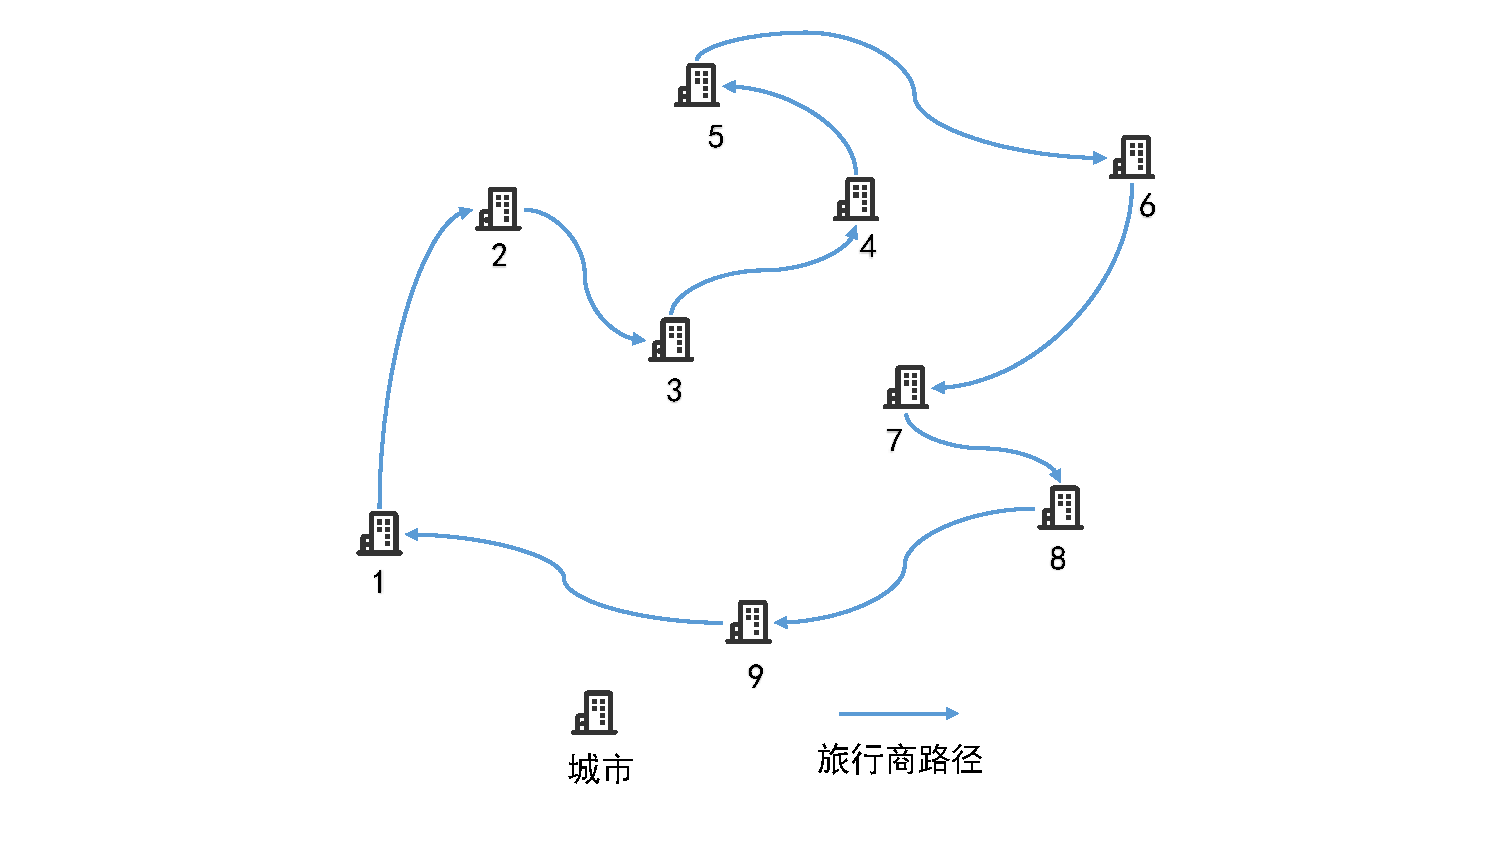
\includegraphics[width=\linewidth]{images/TSP.pdf}\\
    \caption{TSP示意图}
\end{figure}

TSP可以表述为整数线性规划模型\cite{papadimitriou1998combinatorial}:假设共有$N$个城市,每个城市的编号为$1,\cdots,N$,从城市$i$到城市$j$的旅行成本(距离)为$c_{ij}>0$。旅行商的目标是从任意一个城市出发访问完所有的城市,每个城市只能访问一次,最后回到最初的城市,目标是找到一条依次访问所有城市且访问城市不重复的最短路线。TSP中的决策变量为$x_{ij}=\begin{cases}1, & \text{存在从城市$i$到城市$j$的路径}\\0, & \text{其他} \end{cases}$,城市节点集合表示为$V(|V| = N)$。由于可能存在子回路,所以在构建TSP模型时需要消除会产生子回路的情况,这里采用Miller-Tucker-Zemlin (MTZ)约束进行子回路的消除\cite{1960Integer},引入连续变量$u_i(\forall i \in V, u_i \geq 0)$,其取值可以为任何非负实数(实数集合表示为$R$)。这里用$u_i$表示编号为$i$的城市的访问次序,比如当$u_i = 5$时表示编号为1的城市是从出发点开始,第5个被访问到的点。因此,TSP的数学模型可以表示为\crefrange{eq:tsp-obj}{eq:tsp-x_bound}。

\begin{align}
    \min \quad & \sum_{i \in V}\sum_{j \in V, i \neq j} c_{ij}x_{ij} & \label{eq:tsp-obj}\\
    \text{s.t.} \quad & \sum_{i \in V} x_{ij} = 1, & \forall j \in V, i \neq j\label{eq:tsp-in}\\
    \quad & \sum_{j \in V} x_{ij} = 1, & \forall i \in V, i \neq j \label{eq:tsp-out}\\
    \quad & u_i - u_j + Nx_{ij} \leq N - 1, & \forall i, j \in V; i \neq j \label{eq:tsp-subtour}\\
    \quad & u_i \geq 0, & u_i \in R \label{eq:tsp-u_bound}\\
    \quad & x_{ij} \in \{0, 1\}, & i, j \in V; i \neq j \label{eq:tsp-x_bound}
\end{align}

目标函数\eqref{eq:tsp-obj}表示最小化访问所有城市的成本(距离),约束\eqref{eq:tsp-in}和\eqref{eq:tsp-out}保证每个城市节点的入度和出度为1,即每个城市只进入一次和出去一次,保证了每个城市只访问一次,不会被重复访问,约束\eqref{eq:tsp-subtour}消除子回路,约束\eqref{eq:tsp-u_bound}和\eqref{eq:tsp-x_bound}表示变量的取值范围。

%===================================
% 颜色
%===================================
\section{颜色}

% === 测试颜色名称 ===
\subsection{颜色名称测试(dvipsnames, svgnates, x11names)}

\begin{itemize}
    \item \textcolor{Red}{Red (dvipsname)}
    % \item \textcolor{Crimson}{Crimson (svgnames)}
    \item \textcolor{DeepSkyBlue2}{DeepSkyBlue2 (x11names)}
    \item \textcolor{ForestGreen}{ForestGreen (dvipsname)}
    % \item \textcolor{MediumVioletRed}{MediumVioletRed (svgnames)}
    \item \textcolor{DarkOrange1}{DarkOrange1 (x11names)}
\end{itemize}

% === 自定义颜色测试 ===
\subsection{自定义颜色示例}

\definecolor{MyBlue}{RGB}{0, 100, 255} % 使用 RGB 定义颜色
\definecolor{MyYellow}{HTML}{FFD700} % 使用 HTML 十六进制定义颜色

\textcolor{MyBlue}{这是自定义的蓝色文本。}

\textcolor{MyYellow}{这是自定义的黄色文本。}

% === 高级颜色混合测试 ===
\subsection{颜色混合示例}

\textcolor{blue!50!red}{混合 50\% 蓝色和 50\% 红色}

\textcolor{green!60!white}{混合 60\% 绿色和 40\% 白色}

\textcolor{orange!30!yellow!70}{混合 30\% 橙色、70\% 黄色}

% === 背景色测试 ===
\subsection{背景色示例}

% \colorbox{LavenderBlush}{这是 LavenderBlush 背景色的文本。}

\colorbox{SkyBlue}{这是 SkyBlue 背景色的文本。}

% \colorbox{PeachPuff}{这是 PeachPuff 背景色的文本。}

%===================================
% 插入图片及子图测试
%===================================
\section{插入图片及子图}

% === 插入图片测试 ===
\subsection{插入图片}

\begin{figure}[!htb]
    \centering
    
\includegraphics[width=\linewidth]{banner.jpg}\\
    \caption{图片示例}
\end{figure}

% === 子图排列测试 ===
\subsection{子图排列}

\begin{figure}[!htbp]
    % 第一行:两个子图
    \begin{subfigure}[b]{0.48\textwidth}
        
\includegraphics[width=\linewidth]{about.jpg}
        \caption{子图 A}
        \label{fig:subfig_a}
    \end{subfigure}
    \hfill
    \begin{subfigure}[b]{0.48\textwidth}
        
\includegraphics[width=\linewidth]{about.jpg}
        \caption{子图 B}
        \label{fig:subfig_b}
    \end{subfigure}

    % 第二行:两个子图
    \begin{subfigure}[b]{0.48\textwidth}
        
\includegraphics[width=\linewidth]{about.jpg}
        \caption{子图 C}
        \label{fig:subfig_c}
    \end{subfigure}
    \hfill
    \begin{subfigure}[b]{0.48\textwidth}
        
\includegraphics[width=\linewidth]{about.jpg}
        \caption{子图 D}
        \label{fig:subfig_d}
    \end{subfigure}

    \centering
    \caption{多张子图排列示例 1}
    \label{fig:multi_subfigures}
\end{figure}

\begin{figure}[!htbp]
    % 第一行:两个子图
    \begin{subfigure}[b]{\textwidth}
        
\includegraphics[width=\linewidth]{home.jpg}
        \caption{子图 1}
    \end{subfigure}

    % 第二行:两个子图
    \begin{subfigure}[b]{0.48\textwidth}
        
\includegraphics[width=\linewidth]{home.jpg}
        \caption{子图 2}
    \end{subfigure}
    \hfill
    \begin{subfigure}[b]{0.48\textwidth}
        
\includegraphics[width=\linewidth]{home.jpg}
        \caption{子图 3}
    \end{subfigure}

    \centering
    \caption{多张子图排列示例 2}
\end{figure}

%===================================
% 伪代码测试
%===================================
\section{伪代码}

\begin{algorithm}[H]
    \KwIn{This is some input}
    \KwOut{This is some output}
    \SetAlgoLined
    \SetNoFillComment
    \tcc{This is a comment}
    \vspace{3mm}
    some code here\;
    $x \leftarrow 0$\;
    $y \leftarrow 0$\;
    \uIf{$ x > 5$} {
        x is greater than 5 \tcp*{This is also a comment}
    }
    \Else {
        x is less than or equal to 5\;
    }
    \ForEach{y in 0..5} {
        $y \leftarrow y + 1$\;
    }
    \For{$y$ in $0..5$} {
        $y \leftarrow y - 1$\;
    }
    \While{$x > 5$} {
        $x \leftarrow x - 1$\;
    }
    \Return Return something here\;
    \caption{what}
\end{algorithm}

%===================================
% 代码环境测试
%===================================
\section{代码环境}

% === 多行代码测试 ===
\subsection{多行代码}

Python 代码:

\begin{minted}{python}
def hello_en():
    print("Hello, world!")

def hello_cn():
    print("你好,世界!")

hello_en()
hello_cn()
\end{minted}

C++ 代码:

\begin{minted}{cpp}
#include <iostream>
#include <vector>
#include <string>

using namespace std;

void getNext(int *next, const string &p) {
    int m = p.size(), j = 0; // j is the length of the previous longest prefix suffix 
    next[0] = 0; // The first character has no proper prefix or suffix
    for (int i = 1; i < m; ++i) { // Start from the second character
        // Check if the j > 0 because we need to index to the previous next value
        while (j > 0 && p[i] != p[j]) { // Backtrack if there is a mismatch
            j = next[j - 1]; // j - 1 because next is 0-indexed
        }
        if (p[i] == p[j]) { // If characters match, increment j, namely the length of the current prefix
            ++j;
        }
        next[i] = j; // Set the next value for the current character
    }
}

int kmp(const string &s, const string &p) {
    int n = s.size(), m = p.size();
    if (n < m) { // Check if the pattern is longer than the text
        cout << "Pattern is longer than text." << endl;
        return -1;
    }
    if (m == 0) { // Check if the pattern is empty
        cout << "Empty pattern." << endl;
        return -1;
    }
    vector<int> next(m);
    getNext(&next[0], p); // Initialize the next array for the pattern p
    for (int i = 0, j = 0; i < n; ++i) { // i is the index in the main string s and j is the index in the pattern p
        while (j > 0 && s[i] != p[j]) { // Mismatch after j matches
            j = next[j - 1]; // Use the next array to skip unnecessary comparisons, minus 1 because next is 0-indexed
        }
        if (s[i] == p[j]) { // Match found and increment j to check next character
            ++j;
        }
        if (j == m) { // If j equals the length of the pattern, the first occurrence is found
            cout << "Pattern found at index: " << i + 1 - m << endl;
            return 0; // Return after finding the first occurrence
        }
    }
    return -1; // If no match is found, return -1
}

int main() {
    string s, p;
    cin >> s >> p;
    cout << "The main string is: " << s << endl;
    cout << "The pattern string is: " << p << endl;
    int result = kmp(s, p);
    if (result == -1) {
        cout << "Pattern not found." << endl;
    } else {
        cout << "Pattern found successfully." << endl;
    }
    return 0;
}
\end{minted}

% === 行内代码测试 ===
\subsection{行内代码}

This is an example of minted in the same line \mintinline{python}{print("Hello world!")}.

%===================================
% 编辑体验测试 
%===================================
\section{编辑体验}

\subsection{超链接}\label{sec:hyperlink}

The url (outer link) color is just like \href{https://chen-huaneng.github.io/}{this}. The inner link color is just like this one $\rightarrow$ \ref{sec:hyperlink}. The citation is like this\cite{2009A}.

\subsection{脚注}

This is a footnote example\footnote{Related footnote is here.}.

\subsection{边注}

\marginpar{A marginpar.}Such a marginpar is like that. \marginpar{Hello world!} This is after the marginpar.

\subsection{智能交叉引用}

这是一个数学公式引用:\autoref{eq:tsp-out},这是一个图片引用:\autoref{fig:subfig_a},这是一个表格引用:\autoref{tab:fstsp-sign-meaning}。

\section{Section example}

\subsection{Subsection example}

This is a subsection example.

\subsubsection{Subsubsection example}

This is a subsubsection example.

\section*{Unnumbered section example}

\subsection*{Unnumbered subsection example}

This is a unnumbered subsection example.

\subsubsection*{Unnumbered subsubsection example}

This is a unnumbered subsubsection example.

%===================================
% 字体测试
%===================================
\section{中文字体测试}

% === 中文主字体测试 ===
\subsection{中文主字体(LXGWWenKaiScreen)}
这是默认的中文字体(\textbf{加粗}和\textit{斜体}分别为方正黑体和方正楷体)。  
\par
\textbf{加粗文本示例:这是一段加粗的中文文本。}
\par
\textit{斜体文本示例:这是一段斜体的中文文本。}

% === 中文无衬线字体测试 ===
\subsection{中文无衬线字体(FZHTJW)}
{\sffamily
这是无衬线字体(\textbf{加粗}效果由 AutoFake 生成,\textit{斜体}为方正仿宋)。  
\par
\textbf{加粗文本示例:这是一段加粗的无衬线中文文本。}
\par
\textit{斜体文本示例:这是一段斜体的无衬线中文文本。}
}

% === 等宽字体测试 ===
\subsection{等宽字体(LXGWWenKaiMonoScreen)}
{\ttfamily
这是等宽字体(\textbf{加粗}效果由 AutoFake 生成,\textit{斜体}为方正书宋)。  
\par
\textbf{加粗文本示例:这是一段加粗的等宽中文文本。}
\par
\textit{斜体文本示例:这是一段斜体的等宽中文文本。}
}

% === 混合字体测试 ===
\subsection{混合字体测试}
{
\textbf{主字体(LXGWWenKaiScreen)}
\par
\sffamily{无衬线字体(FZHTJW)}
\par
\ttfamily{等宽字体(LXGWWenKaiMonoScreen)}
\par
\textbf{主字体}和\sffamily{无衬线}的切换效果。  
\par
\texttt{等宽字体}与\textbf{普通字体}的对比。 
}

\section{English Font Test}

% === 英文主字体测试 ===
\subsection{English Main Font (Times New Roman)}
This is the default English font (serif).  
\par
\textbf{Bold} and \textit{Italic} effects are generated automatically.  

% === 英文无衬线字体测试 ===
\subsection{English Sans-serif Font (Arial)}
{\sffamily
This is the English sans-serif font.  
\par
\textbf{Bold} and \textit{Italic} effects are generated automatically.  
}

% === 英文等宽字体测试 ===
\subsection{English Monospace Font (Consolas)}
{\ttfamily
This is the English monospace font.  
\par
\textbf{Bold} and \textit{Italic} effects are generated automatically.  
}

% === 混合字体测试 ===
\subsection{中英文混合字体测试}
\textbf{Main Font:} Times New Roman + \textbf{中文主字体:} LXGWWenKaiScreen.  
\par
{\sffamily \textbf{Sans-serif Font:} Arial + \textbf{中文无衬线字体:} FZHTJW.}  
\par
{\ttfamily \textbf{Monospace Font:} Consolas + \textbf{中文等宽字体:} LXGWWenKaiMonoScreen.}

% === 中文字体测试 ===
\section{滕王阁序}
   豫章故郡,洪都新府。星分翼轸(zhěn),地接衡庐。襟三江而带五湖,控蛮荆而引瓯(ōu)越。物华天宝,龙光射牛斗之墟;人杰地灵,徐孺下陈蕃(fān)之榻。雄州雾列,俊采星驰,台隍(huáng)枕夷夏之交,宾主尽东南之美。都督阎公之雅望,棨(qǐ )戟遥临;宇文新州之懿(yì)范,襜(chān )帷(wéi)暂驻。十旬休假,胜友如云;千里逢迎,高朋满座。腾蛟起凤,孟学士之词宗;紫电清霜,王将军之武库。家君作宰,路出名区;童子何知,躬逢胜饯。

  时维九月,序属三秋。潦(lǎo)水尽而寒潭清,烟光凝而暮山紫。俨(yǎn)骖騑(cān fēi)于上路,访风景于崇阿(ē)。临帝子之长洲,得天人之旧馆。层峦耸翠,上出重霄;飞阁流(一作 翔)丹,下临无地。鹤汀(tīng)凫(fú )渚(zhǔ),穷岛屿之萦(yíng)回;桂殿兰宫,即(一作 列)冈峦之体势。

  披绣闼(tà),俯雕甍(méng )。山原旷其盈视,川泽纡(yū)其骇瞩。闾(lǘ)阎(yán) 扑地,钟鸣鼎食之家;舸(gě)舰弥津,青雀黄龙之舳(zhú)。云销雨霁(jì),彩彻区明(或作 虹销雨霁,彩彻云衢 qú)。落霞与孤鹜(wù)齐飞,秋水共长天一色。渔舟唱晚,响穷彭蠡(l ǐ)之滨;雁阵惊寒,声断衡阳之浦。

  遥襟甫畅,逸兴遄(chuán)飞。爽籁发而清风生,纤歌凝而白云遏(è)。睢(suī)园绿竹,气凌彭泽之樽;邺(yè)水朱华,光照临川之笔。四美具,二难并。穷睇眄(dì miǎn)于中天,极娱游于暇日。天高地迥(jiǒng),觉宇宙之无穷;兴尽悲来,识盈虚之有数。望长安于日下,目吴会(kuài)于云间。地势极而南溟(míng)深,天柱高而北辰远。关山难越,谁悲失路之人;萍水相逢,尽是他乡之客。怀帝阍(hūn)而不见,奉宣室以何年。

  嗟(jiē)乎!时运不齐,命途多舛(chuǎn);冯唐易老,李广难封。屈贾谊(yì)于长沙,非无圣主;窜梁鸿于海曲,岂乏明时?所赖君子见机,达人知命。老当益壮,宁移白首之心?穷且益坚,不坠青云之志。酌贪泉而觉爽,处涸辙(hé zhé)以犹欢。北海虽赊(shē),扶摇可接;东隅(yú)已逝,桑榆非晚。孟尝高洁,空余报国之情;阮籍猖狂,岂效穷途之哭!

  勃,三尺微命,一介书生。无路请缨,等终军之弱冠(guàn);有怀投笔,慕宗悫(què)之长风。舍簪(zān)笏(hù)于百龄,奉晨昏于万里。非谢家之宝树,接孟氏之芳邻。他日趋庭,叨(tāo)陪鲤对;今兹捧袂(mèi),喜托龙门。杨意不逢,抚凌云而自惜;钟期既遇,奏流水以何惭?

  呜呼!胜地不常,盛筵(yán)难再;兰亭已矣,梓(zǐ) 泽丘墟。临别赠言,幸承恩于伟饯;登高作赋,是所望于群公。敢竭鄙怀,恭疏短引;一言均赋,四韵俱成。请洒潘江,各倾陆海云尔。 

  滕王高阁临江渚,佩玉鸣鸾罢歌舞。

  画栋朝飞南浦云,珠帘暮卷西山雨。

  闲云潭影日悠悠,物换星移几度秋。

  阁中帝子今何在?槛外长江空自流。

% === 英文字体测试 ===
\section{Do Not Go Gentle into That Good Night}

Do not go gentle into that good night,

Old age should burn and rave at close of day;

Rage, rage against the dying of the light.

Though wise men at their end know dark is right,

Because their words had forked no lightning they

Do not go gentle into that good night.

Good men, the last wave by, crying how bright

Their frail deeds might have danced in a green bay,

Rage, rage against the dying of the light.

Wild men who caught and sang the sun in flight,

And learn, too late, they grieved it on its way,

Do not go gentle into that good night.

Grave men, near death, who see with blinding sight

Blind eyes could blaze like meteors and be gay,   

Rage, rage against the dying of the light.

And you, my father, there on the sad height,

Curse, bless, me now with your fierce tears, I pray.

Do not go gentle into that good night.

Rage, rage against the dying of the light.

%===================================
% 定理盒子测试
%===================================
\section{Theorem, Proposition, Proof}

\begin{theorem}
    If $1<p<\infty$ and $m > n/p$, or $p=1$ and $m \ge n$, there exist a constant $C = C(m,n,\gamma,p)$, such that
    \begin{equation*}
        \Vert R^m u \Vert_{L^\infty(\Omega)} \le C d^{m-n/p} |u|_{W^m_p(\Omega)}
    \end{equation*}
    for all $u \in W^m_p(\Omega)$.
\end{theorem}
\begin{proof}
    First, we assume that $u \in C^m(\Omega) \cap W^m_p(\Omega)$. We can use the pointwise representation of $R^mu(x)$.
    \begin{align*}
        |R^mu(x)| ={} & m \left| \sum_{|\alpha| = m} \int_{C_x} k_{\alpha}(x,z) D^\alpha u(z)\,dz \right| \notag \\
        \le{}         & C \sum_{|\alpha|=m} \int_{\Omega} |x-z|^{-n+m} |D^\alpha u(z)|\,dz \notag                \\
        \le{}         & C' d^{m-n/p} |u|_{W^m_p(\Omega)}.
    \end{align*}
    The proof can be completed via a density argument.
\end{proof}

\begin{theorem}[xxx]
    If $1<p<\infty$ and $m > n/p$, or $p=1$ and $m \ge n$, there exist a constant $C = C(m,n,\gamma,p)$, such that
    \begin{equation*}
        \Vert R^m u \Vert_{L^\infty(\Omega)} \le C d^{m-n/p} |u|_{W^m_p(\Omega)}
    \end{equation*}
    for all $u \in W^m_p(\Omega)$.
\end{theorem}
\begin{proof}[\upshape\bfseries Proof of xxx]
    First, we assume that $u \in C^m(\Omega) \cap W^m_p(\Omega)$. We can use the pointwise representation of $R^mu(x)$.
    \begin{align*}
        |R^mu(x)| ={} & m \left| \sum_{|\alpha| = m} \int_{C_x} k_{\alpha}(x,z) D^\alpha u(z)\,dz \right| \notag \\
        \le{}         & C \sum_{|\alpha|=m} \int_{\Omega} |x-z|^{-n+m} |D^\alpha u(z)|\,dz \notag                \\
        \le{}         & C' d^{m-n/p} |u|_{W^m_p(\Omega)}.
    \end{align*}
    The proof can be completed via a density argument.
\end{proof}

\begin{theorem*}
    If $1<p<\infty$ and $m > n/p$, or $p=1$ and $m \ge n$, there exist a constant $C = C(m,n,\gamma,p)$, such that
    \begin{equation*}
        \Vert R^m u \Vert_{L^\infty(\Omega)} \le C d^{m-n/p} |u|_{W^m_p(\Omega)}
    \end{equation*}
    for all $u \in W^m_p(\Omega)$.
\end{theorem*}
\begin{proof}
    First, we assume that $u \in C^m(\Omega) \cap W^m_p(\Omega)$. We can use the pointwise representation of $R^mu(x)$.
    \begin{align*}
        |R^mu(x)| ={} & m \left| \sum_{|\alpha| = m} \int_{C_x} k_{\alpha}(x,z) D^\alpha u(z)\,dz \right| \notag \\
        \le{}         & C \sum_{|\alpha|=m} \int_{\Omega} |x-z|^{-n+m} |D^\alpha u(z)|\,dz \notag                \\
        \le{}         & C' d^{m-n/p} |u|_{W^m_p(\Omega)}.
    \end{align*}
    The proof can be completed via a density argument.
\end{proof}

\begin{proposition}
    \begin{equation*}
        Q^m u(x) = \sum_{|\lambda| < m} \left( \int_B \psi_\lambda(y) u(y)\,dy \right) x^\lambda
    \end{equation*}
    where $\psi_\lambda \in C_0^\infty(\mathbb{R}^n)$ and $\mathrm{supp}(\phi_\lambda) \in \overline{B}$.
\end{proposition}
\begin{proof}
    This follows from xxx if we define
    \begin{equation*}
        \psi_\lambda(y) = \sum_{\alpha \ge \lambda,|\alpha|<m}
        \frac{(-1)^{|\alpha|}}{\alpha !} a_{[\lambda,\alpha-\lambda]} D^\alpha(y^{\alpha-\lambda} \phi(y)).
    \end{equation*}
\end{proof}

\begin{proposition}[xxx]
    \begin{equation*}
        Q^m u(x) = \sum_{|\lambda| < m} \left( \int_B \psi_\lambda(y) u(y)\,dy \right) x^\lambda
    \end{equation*}
    where $\psi_\lambda \in C_0^\infty(\mathbb{R}^n)$ and $\mathrm{supp}(\phi_\lambda) \in \overline{B}$.
\end{proposition}
\begin{proof}[\upshape\bfseries Proof of xxx]
    This follows from xxx if we define
    \begin{equation*}
        \psi_\lambda(y) = \sum_{\alpha \ge \lambda,|\alpha|<m}
        \frac{(-1)^{|\alpha|}}{\alpha !} a_{[\lambda,\alpha-\lambda]} D^\alpha(y^{\alpha-\lambda} \phi(y)).
    \end{equation*}
\end{proof}

\begin{proposition*}
    \begin{equation*}
        Q^m u(x) = \sum_{|\lambda| < m} \left( \int_B \psi_\lambda(y) u(y)\,dy \right) x^\lambda
    \end{equation*}
    where $\psi_\lambda \in C_0^\infty(\mathbb{R}^n)$ and $\mathrm{supp}(\phi_\lambda) \in \overline{B}$.
\end{proposition*}
\begin{proof}
    This follows from xxx if we define
    \begin{equation*}
        \psi_\lambda(y) = \sum_{\alpha \ge \lambda,|\alpha|<m}
        \frac{(-1)^{|\alpha|}}{\alpha !} a_{[\lambda,\alpha-\lambda]} D^\alpha(y^{\alpha-\lambda} \phi(y)).
    \end{equation*}
\end{proof}

\section{Corollary, Lemma, Claim}

\begin{corollary}
    Under the assumption of xxx, the following inequality holds
    \begin{equation*}
        \inf_{v \in P^{m-1}} \Vert u - v \Vert_{W^k_p(\Omega)} \le C_{m,n,\gamma} d^{m-k} |u|_{W^k_p(\Omega)}, \,\, k = 0,1,\dots,m,
    \end{equation*}
\end{corollary}

\begin{corollary}[xxx]
    Under the assumption of xxx, the following inequality holds
    \begin{equation*}
        \inf_{v \in P^{m-1}} \Vert u - v \Vert_{W^k_p(\Omega)} \le C_{m,n,\gamma} d^{m-k} |u|_{W^k_p(\Omega)}, \,\, k = 0,1,\dots,m,
    \end{equation*}
\end{corollary}

\begin{corollary*}
    Under the assumption of xxx, the following inequality holds
    \begin{equation*}
        \inf_{v \in P^{m-1}} \Vert u - v \Vert_{W^k_p(\Omega)} \le C_{m,n,\gamma} d^{m-k} |u|_{W^k_p(\Omega)}, \,\, k = 0,1,\dots,m,
    \end{equation*}
\end{corollary*}

\begin{lemma}
    Let $f \in L^p(\Omega)$ for $p \ge 1$ and $m \ge 1$ and let
    \[
        g(x) = \int_\Omega |x-z|^{-n+m} |f(z)|\,dz
    \]
    Then
    \begin{equation*}
        \Vert g \Vert_{L^p(\Omega)} \le C_{m,n} d^m \Vert f\Vert_{L^p(\Omega)}.
    \end{equation*}
\end{lemma}

\begin{lemma}[xxx]
    Let $f \in L^p(\Omega)$ for $p \ge 1$ and $m \ge 1$ and let
    \[
        g(x) = \int_\Omega |x-z|^{-n+m} |f(z)|\,dz
    \]
    Then
    \begin{equation*}
        \Vert g \Vert_{L^p(\Omega)} \le C_{m,n} d^m \Vert f\Vert_{L^p(\Omega)}.
    \end{equation*}
\end{lemma}

\begin{lemma*}
    Let $f \in L^p(\Omega)$ for $p \ge 1$ and $m \ge 1$ and let
    \[
        g(x) = \int_\Omega |x-z|^{-n+m} |f(z)|\,dz
    \]
    Then
    \begin{equation*}
        \Vert g \Vert_{L^p(\Omega)} \le C_{m,n} d^m \Vert f\Vert_{L^p(\Omega)}.
    \end{equation*}
\end{lemma*}

\begin{claim}
    $Q^m u$ is a polynomial of degree less than $m$ in $x$.
\end{claim}

\begin{claim}[xxx]
    $Q^m u$ is a polynomial of degree less than $m$ in $x$.
\end{claim}

\begin{claim*}
    $Q^m u$ is a polynomial of degree less than $m$ in $x$.
\end{claim*}

\section{Definition}

\begin{definition}
    $\Omega$ is star-shaped with respect to the ball $B$ if , for all $x \in \Omega$, the closed convex hull of $\{x\} \cup B$ is a subset of $\Omega$.
\end{definition}

\begin{definition}[xxx]
    $\Omega$ is star-shaped with respect to the ball $B$ if , for all $x \in \Omega$, the closed convex hull of $\{x\} \cup B$ is a subset of $\Omega$.
\end{definition}

\begin{definition*}
    $\Omega$ is star-shaped with respect to the ball $B$ if , for all $x \in \Omega$, the closed convex hull of $\{x\} \cup B$ is a subset of $\Omega$.
\end{definition*}

\section{Example}

\begin{example}
    The integral form of the Taylor remainder for $f \in C^m([0,1])$ is given by
    \begin{equation*}
        f(s) = \sum_{k=0}^{m-1}\frac{1}{k!} f^{(k)}(0) + \int_0^s \frac{1}{(m-1)!} f^{(m)}(t)(s-t)^{m-1}\,dt.
    \end{equation*}
\end{example}

\begin{example}[xxx]
    The integral form of the Taylor remainder for $f \in C^m([0,1])$ is given by
    \begin{equation*}
        f(s) = \sum_{k=0}^{m-1}\frac{1}{k!} f^{(k)}(0) + \int_0^s \frac{1}{(m-1)!} f^{(m)}(t)(s-t)^{m-1}\,dt.
    \end{equation*}
\end{example}

\begin{example*}
    The integral form of the Taylor remainder for $f \in C^m([0,1])$ is given by
    \begin{equation*}
        f(s) = \sum_{k=0}^{m-1}\frac{1}{k!} f^{(k)}(0) + \int_0^s \frac{1}{(m-1)!} f^{(m)}(t)(s-t)^{m-1}\,dt.
    \end{equation*}
\end{example*}

\section{Problem, Solution}

\begin{problem}
Calculate the integral of the function $g(x) = 3x^2$ with respect to $x$.
\end{problem}

\begin{solution}
    To calculate the integral of $g(x) = 3x^2$, we use the power rule for integration:
    \[
        \int 3x^2 \, dx = x^3 + C
    \]
    where $C$ is the constant of integration.
\end{solution}

\begin{problem}[xxx]
Calculate the integral of the function $g(x) = 3x^2$ with respect to $x$.
\end{problem}
\begin{solution}[xxx]
    To calculate the integral of $g(x) = 3x^2$, we use the power rule for integration:
    \[
        \int 3x^2 \, dx = x^3 + C
    \]
    where $C$ is the constant of integration.
\end{solution}

\begin{problem*}
    Calculate the integral of the function $g(x) = 3x^2$ with respect to $x$.
\end{problem*}
\begin{solution*}
    To calculate the integral of $g(x) = 3x^2$, we use the power rule for integration:
    \[
        \int 3x^2 \, dx = x^3 + C
    \]
    where $C$ is the constant of integration.
\end{solution*}

\section{Remark}

\begin{remark}
    Such a polynomial is not unique, due to the choice od cut-off function $\phi$.
\end{remark}

\begin{remark}[xxx]
    Such a polynomial is not unique, due to the choice od cut-off function $\phi$.
\end{remark}

\begin{remark*}
    Such a polynomial is not unique, due to the choice od cut-off function $\phi$.
\end{remark*}

\section{Note}

\begin{note}
    The degree of $Q^m u$ is at most $m-1$.
\end{note}

\begin{note}[xxx]
    The degree of $Q^m u$ is at most $m-1$.
\end{note}

\begin{note*}
    The degree of $Q^m u$ is at most $m-1$.
\end{note*}

%===================================
% 参考文献测试
%===================================
\bibliography{references}

\end{document}
